\section{Техническое задание}

\subsection{Основания для разработки}

Основанием для разработки является задание на выпускную квалификационную работу бакалавра "Программное обеспечение для анализа и улучшения аудиозаписей".

\subsection{Цель и назначение разработки}

Создание удобного и функционального инструмента для обработки аудиофайлов с возможностью применения различных звуковых эффектов в реальном времени, визуализации аудиоданных и сохранения результатов обработки. Назначение программы - предоставить пользователям простой в использовании, но мощный инструмент для базовой звуковой обработки, включающий эквалайзер, компрессор и ревербератор, с интуитивно понятным графическим интерфейсом и визуальной обратной связью. Код реализует многопоточную обработку аудио для минимизации задержек, поддерживает загрузку различных аудиоформатов, обеспечивает плавную визуализацию формы волны и частотного спектра, а также предлагает оптимизированные алгоритмы обработки звука. Приложение предназначено для музыкантов, звукорежиссеров и людей, которым требуется быстрый доступ к основным инструментам звуковой обработки без необходимости использования сложных профессиональных DAW.

\subsection{Требования к программно-информационной системе}

\subsubsection{Требования к данным программно-информационной системы}

Входные данные:
\begin{itemize}
	\item аудиофайлы форматов WAV, MP3, OGG, FLAC;
	\item параметры эффектов (эквалайзер, компрессор, реверберация), задаваемые пользователем.
\end{itemize}

Обрабатываемые данные:
\begin{itemize}
	\item аудиосигнал в виде массива numpy.ndarray (форма (N, 1) для моно, (N, 2) для стерео); 
	\item частота дискретизации (стандартно 44100 Гц, но поддерживаются другие значения);
	\item временные и спектральные данные для визуализации (форма волны, частотная характеристика).
\end{itemize}

Выходные данные:
\begin{itemize}
	\item обработанный аудиофайл (экспорт в WAV, MP3);
	\item графики формы сигнала и АЧХ в реальном времени.
\end{itemize}

\subsubsection{Функциональные требования к программно-информационной системе}

В разрабатываемой программе пользователь может:
\begin{itemize}
	\item загружать аудиофайлы разных форматов (wav, mp3, ogg, flac);
	\item экспортировать результат, с применением выбранных им эффектов, в двух форматах: wav и mp3;
	\item воспроизводить, останавливать аудио, изменить позицию воспроизведения, узнать текущее время проигрывания;
	\item применять эффекты в режиме реального времени, включать и отключать их;
	\item применить шумоподавление и настроить его влияние на аудио;
	\item применить эквалайзер, настроить частоты;
	\item применить компрессор, настроить порог, коэффициент сжатия, время атаки и восстановления сигнала, усиление в выбранных диапазонах частот;
	\item применить реверберацию, настроить уровень эффекта, размер комнаты, затухание и чистый звук;
	\item видеть форму сигнала в режиме реального времени, посмотреть АЧХ аудио.
\end{itemize}

\paragraph{Шумоподавление}

Реализовать модуль шумоподавления для аудиопроцессора, обеспечивающий эффективное снижение фонового шума в аудиозаписях с сохранением качества полезного сигнала. Модуль должен поддерживать несколько методов шумоподавления и предоставлять пользователю гибкие настройки степени обработки.

Методы шумоподавления:
\begin{itemize}
	\item спектральное шумоподавление: использовать алгоритм спектрального вычитания шума на основе анализа спектра, автоматическое или ручное определение профиля шума;
	\item медианный фильтр: применять медианный фильтр для удаления импульсных шумов и выбросов;
	\item гауссово размытие: использовать гауссов фильтр для сглаживания сигнала и подавления высокочастотного шума.
\end{itemize}

Управление параметрами:
\begin{itemize}
	\item пользователь должен иметь возможность выбрать метод шумоподавления из списка;
	\item регулировка степени шумоподавления (интенсивность обработки) в диапазоне от 0 (без обработки) до 100 (максимальное подавление);
	\item возможность включения/отключения шумоподавления.
\end{itemize}

Обработка сигнала:
\begin{itemize}
	\item поддержка моно и стерео аудио;
	\item обработка должна выполняться в реальном времени или офлайн с минимальной задержкой;
	\item сохранение временной структуры и качественных характеристик полезного сигнала;
	\item предотвращение появления артефактов (искажений, «водянистости» звука).
\end{itemize}

\paragraph{Эквалайзер}

Реализовать цифровой эквалайзер как часть аудиопроцессора для интерактивной обработки музыкальных и речевых аудиофайлов. Эквалайзер должен обеспечивать гибкую настройку амплитудно-частотной характеристики сигнала в реальном времени с возможностью визуализации.

Функциональные требования:
\begin{itemize}
	\item эквалайзер должен состоять из 8 полос с фиксированными центральными частотами: 50 Гц, 150 Гц, 250 Гц, 500 Гц, 1 кГц, 3 кГц, 7 кГц, 15 кГц;
	\item для каждой полосы пользователь должен иметь возможность регулировать усиление/ослабление в диапазоне от -12 дБ до +12 дБ с шагом не менее 0.1 дБ;
	\item усиление/ослабление должно применяться к соответствующему частотному диапазону без существенных фазовых искажений и без возникновения паразитных резонансов;
	\item для каждой полосы должны быть реализованы цифровые фильтры второго порядка Баттерворта:
	\begin{itemize}
		\item для самой низкой полосы (50 Гц) — lowpass фильтр;
		\item для самой высокой полосы (15 кГц) — highpass фильтр;
		\item для остальных полос — bandpass фильтры с шириной полосы ± 20 процентов от центральной частоты;
	\end{itemize}
	\item все фильтры должны рассчитываться динамически в зависимости от текущей частоты дискретизации аудиосигнала;
	\item фильтры должны быть реализованы с помощью функций butter и lfilter из библиотеки scipy.signal;
	\item для ускорения работы коэффициенты фильтров должны кэшироваться и пересчитываться только при изменении параметров;
	\item итоговый сигнал должен формироваться как сумма результатов обработки всех полос;
	\item эквалайзер должен поддерживать обработку как моно, так и стерео сигналов;
	\item необходимо реализовать функцию визуализации амплитудно-частотной характеристики (АЧХ) эквалайзера в реальном времени;
	\item все параметры эквалайзера должны быть доступны для программного и пользовательского управления (через API и/или GUI).
\end{itemize}

Эквалайзер должен быть реализован с приоритетом качества звука, стабильности работы и удобства пользовательского управления параметрами. Вся логика фильтрации и суммирования полос должна быть максимально прозрачна для дальнейшей доработки и интеграции с другими эффектами аудиопроцессора.

\paragraph{Компрессор}

Реализовать цифровой многополосный компрессор для обработки аудиосигнала в составе аудиопроцессора. Компрессор должен обеспечивать независимую динамическую обработку трёх частотных диапазонов (low, mid, high) с индивидуальными настройками и возможностью визуализации изменений сигнала.

Компрессор должен обеспечивать обработку аудиосигнала в трёх частотных диапазонах с возможностью регулировки и настройки:
\begin{itemize}
	\item low Band: 20–200 Гц;
	\item mid Band: 200–3000 Гц;
	\item high Band: 3000–20000 Гц.
\end{itemize}

Для каждого диапазона должны быть реализованы следующие параметры, доступные для настройки:
\begin{itemize}
	\item threshold (порог срабатывания): от -60 дБ до 0 дБ с шагом не менее 0.1 дБ;
	\item ratio (степень сжатия): от 1:1 до 20:1.;
	\item attack (время атаки): от 0.1 до 500 мс;
	\item release (время восстановления): от 1 до 1000 мс;
	\item makeup gain (дополнительное усиление): от -12 до +12 дБ;
	\item soft knee (мягкость перехода): от 0 до 24 дБ;
	\item bypass (включение/выключение полосы).
\end{itemize}

Компрессор должен корректно работать с моно и стерео сигналами.

Для разделения сигнала на полосы должны использоваться цифровые фильтры (Butterworth или аналогичные) с динамическим расчётом коэффициентов в зависимости от частоты дискретизации.

Основные параметры компрессии:
\begin{enumerate}
	\item Threshold (порог) измеряется в dB - определяет уровень входного сигнала в децибелах, при превышении которого компрессор начинает снижать громкость. Чем ниже порог, тем больше сигнал подвергается сжатию.
	\item Ratio (коэффициент компрессии) – задает отношение входного превышения порога к выходному уровню сигнала. Например, при ratio 4:1, если входной сигнал превышает порог на 4 дБ, то выходной уровень будет превышать порог только на 1 дБ. Диапазон обычно от 1:1 (без сжатия) до 20:1 и выше. Чем выше ratio, тем сильнее сжатие.
	\item Attack (атака) – время в миллисекундах, за которое компрессор начинает снижать уровень сигнала после превышения порога. Быстрая атака позволяет быстро подавлять пики, медленная — сохраняет естественную атаку звука, например, ударных.
	\item Release (восстановление) – время в миллисекундах, за которое компрессор возвращается к нормальному усилению после того, как уровень сигнала опускается ниже порога. Более медленное восстановление создаёт плавное звучание, быстрое — более динамичное.
	\item Knee (характеристика перехода) – определяет плавность начала сжатия вокруг порога. При значении 0 dB компрессия начинается резко (hard knee), при увеличении до 24 dB — плавно (soft knee), что делает переход менее заметным и звучание более естественным.
	\item Make-up Gain (компенсационное усиление) – усиление выходного сигнала после сжатия для компенсации потерь громкости. Измеряется в децибелах. Позволяет вернуть общий уровень громкости на желаемый уровень.
\end{enumerate}

Для оптимизации производительности и работы в реальном времени использованы:
\begin{itemize}
	\item JIT-компиляция критических участков (Numba);
	\item векторизированные вычисления (NumPy);
	\item параллельная обработка полос;
	\item кэширование коэффициентов фильтров.
\end{itemize}

Формулы вычисления сигнала:
\begin{enumerate}
	\item Threshold (порог срабатывания). Порог задаётся в децибелах (dB) и служит уровнем, при превышении которого начинается компрессия. Если амплитуда сигнала в линейной шкале — A, то уровень в децибелах: L = 20 log10(A). Порог T задан в децибелах. Компрессор начинает сжимать сигнал, когда:	L > T.
	\item Ratio (степень компрессии). Определяет, насколько сильно уменьшается превышение уровня сигнала над порогом. Если входной уровень выше порога на ΔL = L − T, то выходной уровень превышения будет: ΔLout = T + ΔL/R, где - R - коэффициент компрессии (ratio).
	\item Attack и Release (время атаки и восстановления). a/r = e**(-1/t*fs), где a/r - атака/восстановление, t - время атаки или релиза в секундах, fs - частота дискретизации. Коэффициент усиление g[n] обновляется так: g[n] = a * g[n-1] + (1 - a) * gt[n], если gt[n] < g[n-1], g[n] = r * g[n-1] + (1 - r) * gt[n], если gt[n] >= g[n-1], где gt[n] - целевой коэффициент усиленияБ вычисляемый по уровню сигнала и ratio.
	\item Knee Width (ширина колена). Для входного уровня L, порога T и ширины колена W, вычисляем коэффициент усиления G в децибелах так:
	\begin{itemize}
		\item если L < T - W/2, то компрессия не применяется: G = 0;
		\item если L > T + W/2, применяется полное сжатие: G = T + (L - T)/R - L;
		\item если T - W/2 <= L <= T + W/2, плавный переход с помощью квадратичной функции: Δ = L - (T - W/2), G = ((1/R - 1) Δ**2)/2W.
	\end{itemize}
	\item Makeup Gain (усиление после компрессии). Если G — makeup gain в децибелах, то коэффициент усиления в линейной шкале: G = 10**(G/20). Итоговый выходной сигнал: y[n] = x[n] * g[n] * G, где y[n] — выходной сигнал на сэмпле n, x[n] — входной сигнал на сэмпле n, g[n] — коэффициент усиления компрессора (динамическое уменьшение или увеличение уровня) на сэмпле n.
\end{enumerate}

Компрессор должен быть реализован с приоритетом качества звука, стабильности работы и удобства пользовательского управления параметрами. Вся логика фильтрации, разделения на полосы и динамической обработки должна быть максимально прозрачна для дальнейшей доработки и интеграции с другими эффектами аудиопроцессора.

\paragraph{Реверберация}

Реализовать алгоритм реверберации Moorer для аудиопроцессора, имитирующий акустику помещений с настраиваемыми параметрами. Алгоритм должен сочетать ранние отражения (early reflections) и поздний реверберационный хвост (late reverb), обеспечивая естественное пространственное звучание.

Основные параметры:
\begin{enumerate}
	\item Размер помещения (Room Size): диапазон: 0.1 (малая комната) – 2.0 (большой зал). влияет на плотность и задержку ранних отражений/хвоста.
	\item Соотношение Wet/Dry: Диапазон: 0 (только сухой сигнал) – 100 (только реверберация).
	\item Демпфирование (Damping): Диапазон: 0 (полное отражение ВЧ) – 100 (сильное подаление ВЧ). Регулирует затухание высоких частот в хвосте.
	\item Pre-Delay: диапазон: 0–200 мс. Задержка перед началом реверберации для имитации расстояния до стен.
\end{enumerate}

Техническая реализация:
\begin{itemize}
	\item использование кольцевого буфера (delay line) для обработки задержек;
	\item оптимизация вычислений через JIT-компиляцию (Numba) для работы в реальном времени;
	\item поддержка моно и стерео сигналов;
	\item кэширование коэффициентов фильтров при изменении параметров.
\end{itemize}

\paragraph{Визуализация}

Реализовать модуль визуализации аудиосигнала, обеспечивающий отображение формы волны и амплитудно-частотной характеристики (АЧХ) в реальном времени. Модуль предназначен для наглядного представления динамики и спектрального состава звука, облегчая анализ и настройку аудиоэффектов.

Визуализация формы волны:
\begin{itemize}
	\item отображать временную амплитуду аудиосигнала (осциллограмму) с возможностью масштабирования по времени и амплитуде;
	\item поддержка моно и стерео сигналов с разделением каналов;
	\item обновление визуализации в реальном времени с частотой не менее 30 кадров в секунду;
	\item обеспечить плавное и без мерцаний отображение;
	\item возможность отображения как полного сигнала, так и его текущего фрагмента (окна).
\end{itemize}

Визуализация амплитудно-частотной характеристики (АЧХ):
\begin{itemize}
	\item расчёт спектра аудиосигнала с использованием быстрого преобразования Фурье (FFT);
	\item отображение амплитуды частотного спектра в логарифмическом или линейном масштабе по оси частот (от 20 Гц до 20 кГц);
	\item обновление спектра в реальном времени с возможностью регулировки оконного размера FFT для баланса между частотным и временным разрешением;
	\item поддержка отображения спектра для каждого канала отдельно (в случае стерео);
	\item визуализация текущих настроек эквалайзера и эффектов (например, наложение АЧХ эквалайзера).
\end{itemize}

\paragraph{Управление}

Реализовать модуль управления аудиопроцессором, обеспечивающий интерактивное управление воспроизведением, настройкой параметров аудиоэффектов и навигацией по аудиофайлам через графический интерфейс и программный API.

Управление воспроизведением:
\begin{itemize}
	\item кнопки Play и Stop для запуска и остановки воспроизведения аудиофайла;
	\item ползунок (слайдер) для перемотки и точного позиционирования в аудио;
	\item отображение текущей позиции воспроизведения и общей длительности аудиофайла;
	\item поддержка управления воспроизведением в реальном времени без задержек.
\end{itemize}

Управление параметрами эффектов:
\begin{itemize}
	\item регулировка параметров эквалайзера (8 полос): усиление/ослабление каждой полосы в диапазоне ±12 дБ;
	\item управление параметрами многополосного компрессора: threshold, ratio, attack, release, makeup gain, soft knee для каждой полосы (low, mid, high);
	\item настройка параметров реверберации: wet/dry, room size, damping;
	\item выбор и регулировка параметров шумоподавления (метод, интенсивность);
	\item все регуляторы должны быть реализованы через удобные элементы управления (ползунки, кнопки, вращающиеся регуляторы).
\end{itemize}

Состояния и обратная связь:
\begin{itemize}
	\item отображение текущих значений параметров в интерфейсе;
	\item обеспечение мгновенного отклика интерфейса на изменение параметров;
	\item индикация состояния воспроизведения (воспроизводится/пауза/стоп);
	\item защита от некорректных значений параметров (валидация ввода).
\end{itemize}

\subsubsection{Моделирование вариантов использования}

На рисунке \ref{fig:use_case_diagram} изображена диаграмма прецедентов

\begin{figure}[ht]
	\center{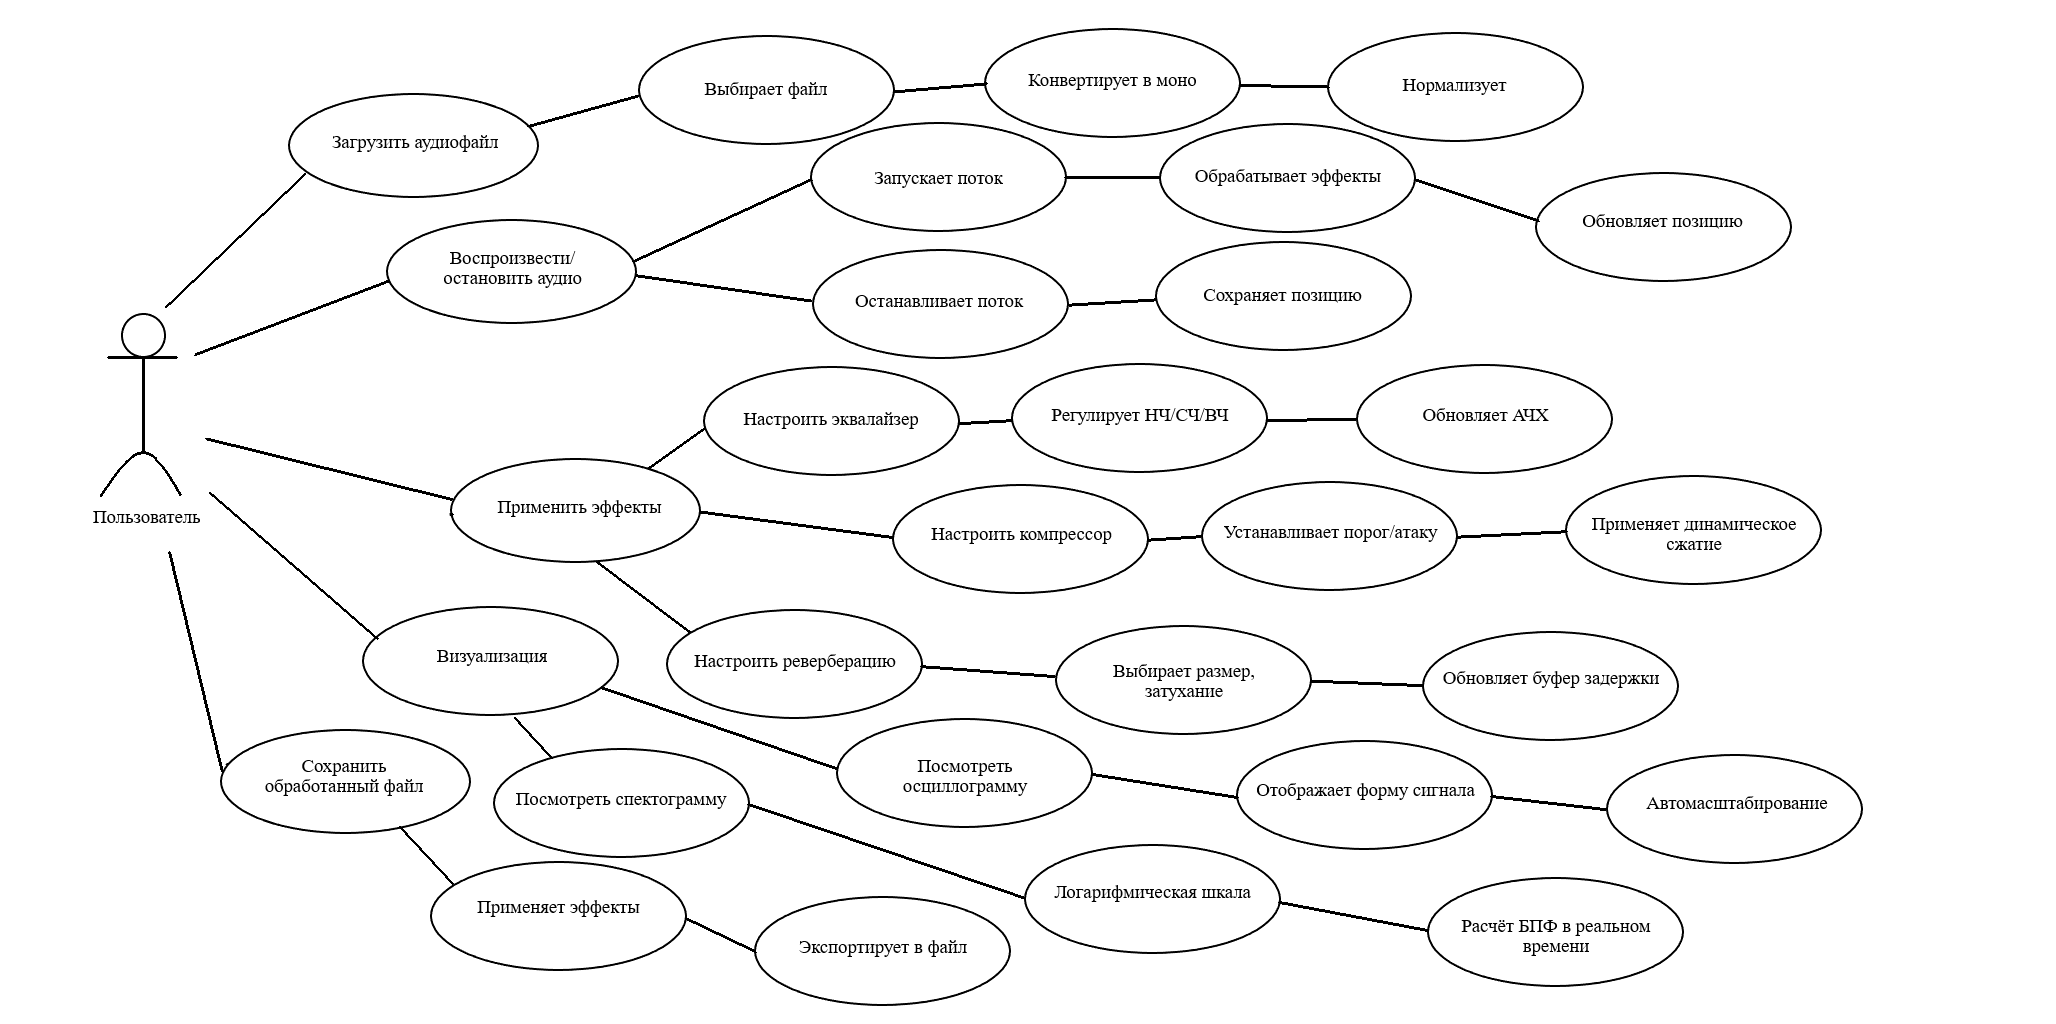
\includegraphics[width=1\linewidth]{DiagramPrec}}
	\caption{Диаграмма прецедентов}
	\label{fig:use_case_diagram}
\end{figure}

\paragraph{Вариант использования «Загрузка аудиофайла»}
Заинтересованные лица и их требования: пользователь хочет загрузить аудиофайл для последующей обработки.

Требования: поддержка форматов (WAV, MP3, OGG, FLAC), автоматическая конвертация в моно, нормализация амплитуды.

Предусловие: приложение запущено, файл существует и доступен для чтения.

Постусловие: аудиоданные загружены в память, форма волны отображена на графике, кнопки "Воспроизвести" и "Сохранить" активированы.

Основной успешный сценарий:
\begin{enumerate}
	\item Пользователь нажимает кнопку "Загрузить".
	\item Открывается диалоговое окно выбора файла.
	\item Пользователь выбирает файл и подтверждает выбор.
\end{enumerate}

\paragraph{Вариант использования «Воспроизведение аудио»}

Заинтересованные лица и их требования: пользователь хочет прослушать загруженный файл с возможностью применения эффектов в реальном времени.

Предусловие: аудиофайл успешно загружен, аудиоустройство вывода доступно.

Постусловие: аудиопоток запущен, графики обновляются в реальном времени.

Основной успешный сценарий:
\begin{enumerate}
	\item Пользователь нажимает кнопку «Воспроизвести».
	\item Система инициализирует аудиопоток.
	\item Callback-функция начинает передавать данные в устройство.
	\item Позиция воспроизведения обновляется каждые 100 мс.
	\item Сигнал и АЧХ отображаются в реальном времени.
\end{enumerate}

\paragraph{Вариант использования «Остановка воспроизведения»}

Заинтересованные лица и их требования: пользователь хочет немедленно прекратить воспроизведение аудио.

Предусловие: идёт воспроизведение аудиофайла.

Постусловие: аудиопоток полностью остановлен, интерфейс обновлен.

Основной успешный сценарий:
\begin{enumerate}
	\item Пользователь нажимает кнопку "Стоп".
	\item Система останавливает воспроизведение аудио.
	\item Текущая позиция фиксируется для возможности дальнейшего продолжения.
\end{enumerate}

\paragraph{Вариант использования «Изменения позиции воспроизведения»}

Заинтересованные лица и их требования: пользователь хочет перемотать аудио на произвольную позицию.

Предусловие: аудиофайл загружен.

Постусловие: текущая позиция воспроизведения изменена, при активном воспроизведении звук продолжается с новой позиции, интерфейс синхронизирован.

Основной успешный сценарий:
\begin{enumerate}
	\item Пользователь перемещает ползунок позиции мышью.
	\item Система пересчитывает позицию.
	\item При воспроизведении поток начинает чтение с новой позиции.
\end{enumerate}

\paragraph{Вариант использования «Применения шумоподавления»}

Заинтересованные лица и их требования: пользователь хочет уменьшить фоновый шум в аудиозаписи для улучшения качества звучания.

Предусловие: файл загружен, кнопка «Шумоподавление» нажата.

Постусловие: выбранный метод шумоподавления и степень обработки применены к аудиопотоку, визуализация обновлена.

Основной успешный сценарий:
\begin{enumerate}
	\item Пользователь активирует кнопку «Шумоподавление».
	\item Выбирает метод шумоподавления из выдвижного списка (спектральное, медианный фильтр, гауссово размытие).
	\item Регулирует интенсивность шумоподавления с помощью knob.
	\item Система применяет выбранный алгоритм с заданной интенсивностью к аудиосигналу.
	\item Обновляется визуализация формы волны и АЧХ.
\end{enumerate}

\paragraph{Вариант использования «Применения эквалайзера»}

Заинтересованные лица и их требования: пользователь хочет настроить частотный баланс (НЧ/СЧ/ВЧ).

Предусловие: файл загружен, вкладка "Эквалайзер" открыта.

Постусловие: параметры эквалайзера применены к аудиопотоку, график АЧХ обновлен.

Основной успешный сценарий:
\begin{enumerate}
	\item Пользователь включает чекбокс «Эквалайзер».
	\item Регулирует ползунки НЧ/СЧ/ВЧ.
	\item Система пересчитывает коэффициент БИХ-фильтров.
	\item Аудиозапись изменяется в соответствии с настройками пользователя.
	\item АЧХ отображается на графике.
\end{enumerate}

\paragraph{Вариант использования «Применения компрессора»}

Заинтересованные лица и их требования: пользователь хочет изменить динамический диапазон аудиосигнала для более равномерного звучания.

Предусловие: аудиофайл успешно загружен, вкладка "Компрессор" открыта.

Постусловие: параметры компрессора применены к аудиопотоку, изменения слышны при воспроизведении.

Основной успешный сценарий:
\begin{enumerate}
	\item Пользователь активирует чекбокс «Компрессор».
	\item Устанавливает диапазон обработки частот для каждого из трёх фильтров.
	\item Устанавливает порог, коэффициент компрессии, время атаки и восстановления, усиление выходного сигнала.
	\item Аудио обрабатывается в режиме реального времени.
\end{enumerate}

\paragraph{Вариант использования «Применения реверберации»}

Заинтересованные лица и их требования: пользователь хочет добавить эффект реверберации к аудиосигналу.

Предусловие: аудиофайл успешно загружен, вкладка "Реверберация" открыта.

Постусловие: эффект реверберации применен к аудиопотоку, буфер реверберации инициализирован с новыми параметрами.

Основной успешный сценарий:
\begin{enumerate}
	\item Пользователь активирует чекбокс "Реверберация".
	\item Пользователь регулирует параметры: уровень эффекта, исходный звук, размер комнаты, затухание.
	\item Аудио обрабатывается в режиме реального времени.
\end{enumerate}	

\paragraph{Вариант использования «Сохранение обработанного файла»}

Заинтересованные лица и их требования: пользователь хочет экспортировать результат с примененными эффектами.

Предусловие: файл загружен, эффекты настроены.

Постусловие: файл сохранен на диск в выбранном формате.

Основной успешный сценарий:
\begin{enumerate}
	\item Пользователь нажимает "Сохранить".
	\item Открывается диалог выбора формата (WAV/MP3) и пути.
	\item Пользователь выбирает формат, путь и название файла.
	\item Система применяет выбранные эффекты, экспортирует файл.
	\item Файл успешно сохранён на диске.
\end{enumerate}		

\paragraph{Вариант использования «Визуализация данных»}

Заинтересованные лица и их требования: пользователь хочет видеть графическое представление аудиосигнала.

Предусловие: аудиофайл загружен и идет воспроизведение.

Постусловие: графики формы волны и АЧХ отображаются и обновляются в режиме реального времени.

Основной успешный сценарий:
\begin{enumerate}
	\item Пользователь нажимает «Воспроизвести».
	\item Система отображает графики формы волны и АЧХ.
\end{enumerate}	

%--------------------------------------------------------------------------------------------------------

\subsection{Требования пользователя к интерфейсу приложения}

Приложение должно иметь следующие основные функции:
\begin{enumerate}
	\item Основные элементы управления - кнопки управления воспроизведением: "Загрузить", "Воспроизвести", "Стоп", "Сохранить". Ползунок позиции воспроизведения, точное позиционирование, индикатор текущей позиции в формате MM:SS / MM:SS.
	\item Визуализация аудио - два синхронизированных графика: верхний график формы волны и нижний график амплитудно-частотной характеристики. Подписи осей с единицами измерения (амплитуда, частота).
	\item Кнопка "Шумоподавление" с двумя положениями: активно/неакитвно, выплывающий список с выбором метода, регулировка интенсивности шумоподавления.
	\item Панель эффектов (вкладки):
	\begin{enumerate}
		\item Эквалайзер - Три ползунка с подписями: низкие частоты (150Hz): ±24 дБ, средние частоты (1kHz): ±24 дБ, высокие частоты (5kHz): ±24 дБ. Чекбокс активации эффекта.
		\item Компрессор - ползунки параметров: порог: -60..0 дБ, соотношение: 1..20, атака: 1..500 мс, восстановление: 10..2000 мс, усиление: 0..24 дБ. Панель отображения диапазонов изменения и применения параметров, а так же ползунки настройки и регулировки диапзаонов. Чекбокс активации эффекта. 
		\item Реверберация: ползунки параметров: уровень эффекта: 0..1, сухой сигнал: 0..1, размер помещения: 0.1..2.0, затухание: 0.1..0.9. Чекбокс активации эффекта.
	\end{enumerate}	
	\item Обратная связь и состояние: индикатор загрузки при обработке файлов. Всплывающие уведомления об ошибках: при неудачной загрузке файла, при проблемах с аудиоустройством, при ошибках сохранения. Изменение состояния кнопок: "Воспроизвести" активна только при загруженном файле, "Стоп" активна только во время воспроизведения, "Сохранить" активна только после загрузки файла.
	\item Производительность: задержка отклика интерфейса не более 100 мс, плавная анимация графиков без рывков, минимальное потребление ресурсов в фоновом режиме.
\end{enumerate}	

\subsubsection{Нефункциональные требования к программно-информационной системе}

\paragraph{Требования к надёжности}

В процессе работы аудио-процессора могут возникнуть следующие аварийные ситуации:
\begin{itemize}
	\item потеря доступа к аудиоустройству в связи с его отключением, изменением системных настроек звука или конфликтом с другим приложением;
	\item попытка загрузки повреждённого или неподдерживаемого аудиофайла с несовместимым форматом, битрейтом или частотой дискретизации;
	\item неожиданное прекращение работы из-за нехватки системных ресурсов при обработке объёмных файлов или одновременном применении нескольких ресурсоёмких эффектов;
	\item ошибки в работе эффектов обработки звука, приводящие к искажению аудиосигнала или сбоям в воспроизведении.
\end{itemize}

Приложение должно автоматически определять доступные аудиоустройства и переключаться между ними при потере соединения с текущим устройством. В случае невозможности восстановления подключения система должна сохранять возможность обработки звука без функции воспроизведения с уведомлением пользователя о возникшей проблеме.

Для работы с аудиофайлами приложение должно проверять их целостность и соответствие поддерживаемым форматам перед загрузкой, а также автоматически выполнять необходимые преобразования (нормализацию, конвертацию в моно, приведение к стандартной частоте дискретизации). При обнаружении критических ошибок в файле пользователь должен получить понятное сообщение о проблеме с указанием конкретной причины.

Для предотвращения аварийного завершения из-за нехватки ресурсов система должна контролировать использование оперативной памяти и процессорного времени, ограничивать размеры буферов обработки и корректно завершать работу при приближении к предельным значениям. Все параметры эффектов и текущее состояние обработки должны сохраняться даже при аварийном завершении работы.

При возникновении ошибок в работе эффектов обработки звука система должна автоматически сбрасывать параметры эффектов к безопасным значениям, сохраняя при этом возможность дальнейшей работы. Все критические ошибки должны фиксироваться в системном логе с указанием времени возникновения, типа ошибки и состояния системы на момент сбоя.

\paragraph{Требования к безопасности}

Требования к приложению:
\begin{enumerate}
	\item Перед загрузкой файла, система должна проверять формат и корректность заголовков. При обнаружении повреждённых данных программа будет выводить ошибку без попытки обработки.
	\item Для безопасности управления памятью и ресурсами необходима изоляция обработки аудио, то есть каждый эффект будет применяться в отдельном потоке с контролем потребления ресурсов и будет ограничен буфе. Так же потребуется очистка временных данных, чтобы после завершения обработки или при ошибке все промежуточные буферы будут очищаться.
	\item Для защиты от вирусов применится проверка структуры файлов, анализ сигнатуры файла перед декодированием, ограничение максимальной длительности обрабатываемого аудио.
	\item Пользовательские настройки будут проверятся перед применением, а недопустимые значения автоматически скорректируются до ближайших безопасных.
	\item При завершении работы, приложение будет останавливать все потоки, освобождать аудиоустройства.
\end{enumerate}

\paragraph{Требования к программному обеспечению}

Для реализации программы будет использоваться язык программирования Python и библиотеки: NumPy, SciPy, PyDub, SoundDevice, Matplotlib, Numba.

Для работы приложения требуется Windows 10/11 (64-bit)

\paragraph{Требования к аппаратному обеспечению}

Минимальная конфигурация:

Центральный процессор с количеством ядер от 2 и выше с тактовой частотой от 2.0 ГГц. Поддержка инструкций SSE4.2. Оперативная память - 4 ГБ. 100 МБ свободного места для установки. Поддержка ASIO/WASAPI для профессионального использования.

\subsubsection{Требования к оформлению документации}

Разработка программной документации и программного изделия должна производиться согласно ГОСТ 19.102-77 и ГОСТ 34.601-90. Единая система программной документации.